\chapter{系统设计}
本章给出了本文设计的非对称半桥反激式变换器系统的性能和设计指标。 首先给出了本文设计的AHB变换器的性能指标,介绍了控制芯片的内部原理图。此外, 为了提高系统的转换效率,分析了反激式变换器的主要损耗,总结了影响系统损耗的主要因素。根据损耗分析的结果,设计了多模式的控制方案,通过系统的带载情况来调节变换器的开关频率和原边的峰值电流值,从而降低系统的损耗,实现系统的整体效率的提升。另外,为了进一步提高系统的转换效率,针对性的提出了两种关键技术,分别用以降低功率管开关损耗和变压器的传导损耗。除此之外,为了降低系统的待机功耗,设计了空载下的突发工作模式。最后为了保证变换器能够稳定的运行,设计了副边反馈网络的二阶补偿结构,并对系统进行了稳定性仿真。


\section{外部电路结构}
本文设计的非对称半桥反激式开关电源变换器的外部电路结构如图所示,包括输入整流回路和反馈回路,为了提高反馈精度,反激回路采用副边反馈结构,通过TL431和光耦模块直接对输出电压进行采样产生误差信号反馈给变换器芯片来为稳定输出电压。

输入回路包扩输入整流滤波和片外启动电路两部分,输入整流滤波由四个二极管和电容Cdc组成,将从电网传递进来的交流信号Vac经过整流滤波后转换为直流输入信号Vdc,此输入信号是一个直流的高压,无法直接为变换器芯片进行供电,通过电阻R1和R2分压后给变换器芯片供电,当其超过片内欠压锁定电路的最低电压后芯片开始工作,随着芯片控制高低边功率管的来回通断,辅助绕组能量积攒到一定程度后,二极管D2导通,对电容Cvdd进行充电,产生变换器输入电压Vdd,代替输入信号Vdc的分压信号稳定地为变换器芯片电源端进行供电。


\section{系统架构}

\subsection{芯片特点和设计指标}

• 支持宽输入电压范围

• 支持宽输出电压范围

• 高效多模式控制

• 轻载低功耗模式

• 全电压和负载条件下支持零电压导通

\begin{table}[htbp]
    \caption{控制芯片的引脚定义}
    \label{tab:控制芯片的引脚定义}
    \centering
    \belowrulesep=0pt  %防止竖线不连续
    \aboverulesep=0pt  %防止竖线不连续
        \begin{tabular}{c|c|c}
            \toprule
            引脚标号 & 名称 & 功能  \\
            \midrule
            1 & EN   & 使能端                                              \\  \midrule
            2 & VDD  & 变换器芯片内部供电端                                 \\  \midrule
            3 & HSGD & 半桥变换器高边功率管的栅极驱动器,控制高边功率管的通断  \\\midrule  
            4 & LSGD & 半桥变换器高边功率管的栅极驱动器,控制低边功率管的通断  \\\midrule  
            5 & ZCD  & 辅助绕组分压采样端                                    \\  \midrule
            6 & CS   & 变压器原边峰值电流采样端                               \\ \midrule
            7 & VS   & 输入电压分压端                                        \\  \midrule
            8 & GND  & 变换器芯片接地端                                      \\  \midrule
            9 & HB   & 功率管半桥中间节点端                                   \\ 
              
            \bottomrule
        \end{tabular}
\end{table}

\subsection{芯片内部结构}
图给出了芯片内部结构架构,该架构包括电源模块、峰值电流控制模块、 退磁检测模块、前沿消隐模块、精确谷底导通模块、谷值锁定模块、前沿消隐(LEB)、退磁时间逐步逼近模块、模式选择模块、逻辑控制模块和驱动等主要模块,每个模块的功能定义如下:

\begin{figure}[htbp] 
    \centering
    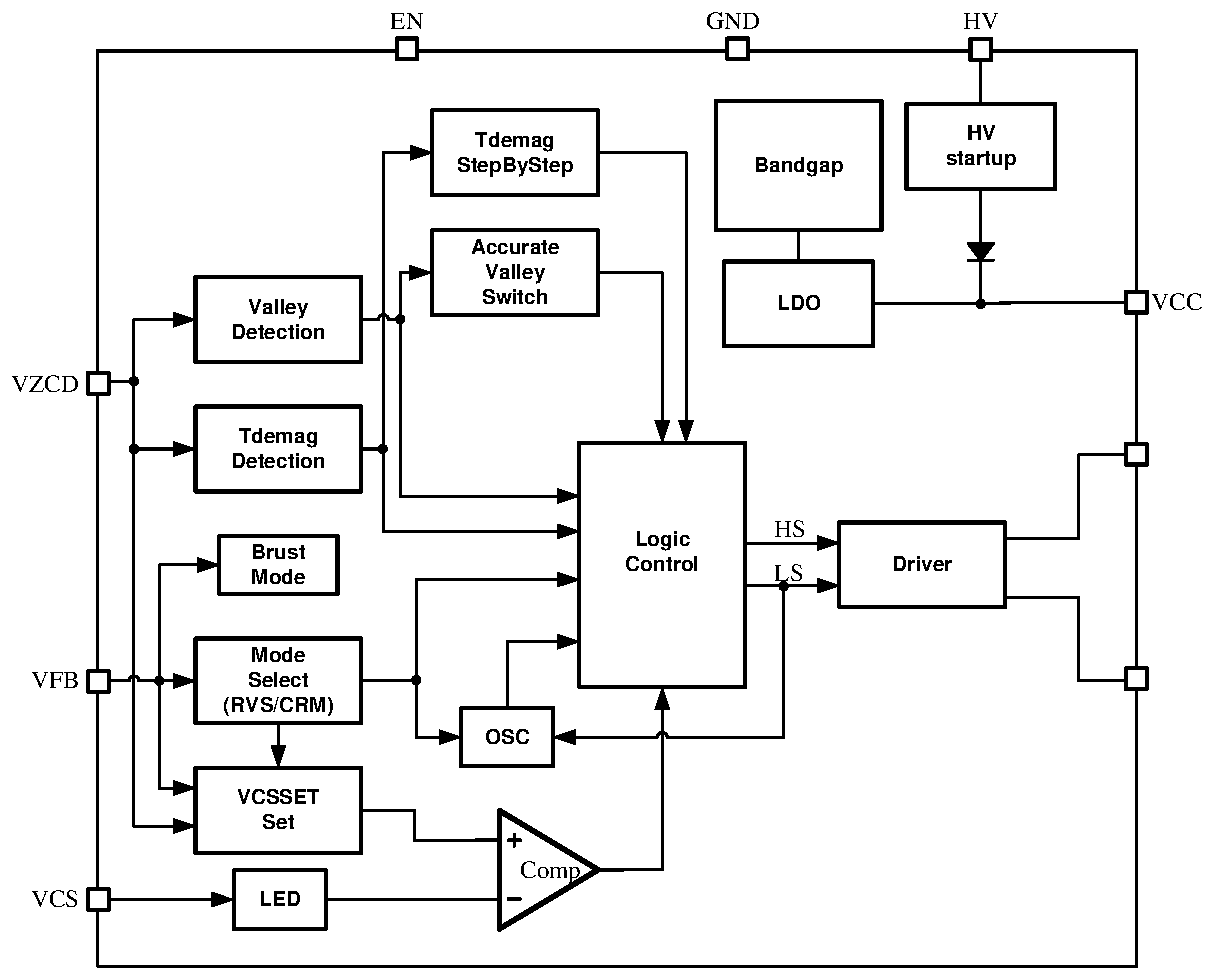
\includegraphics[width=0.8\linewidth]{figures/芯片内部结构图.pdf}
    \caption{芯片内部结构图}
    \label{fig:芯片内部结构图}
\end{figure}

\textbf{电源模块}:电源模块主要包括芯片的欠压锁定电路、带隙基准和降压电路等,该模块的主要作用是为芯片内部各个模块提供稳定的供电电压和各种不受PVT影响的精确偏置电压信号。

\textbf{峰值电流控制模块}:峰值电流控制模块通过对片外副边反馈信号$V_{FB}$和辅助绕组分压信号$V_{ZCD}$进行配置补偿后,产生对应的峰值电流信号Vcspeak,用于和采样电阻上的采样电压信号Vcs进行比较控制高边功率管的导通和关断;该模块的主要功能是为了满足非对称半桥反激式开关电源变换器的宽输出范围下产生相对应的峰值电流信号Vcspeak,防止副边反馈信号$V_{FB}$在不同输出电压相同负载条件下的不匹配,影响后续电路的模式选择控制。

\textbf{退磁检测模块}:退磁检测模块将辅助绕组分压信号$V_{ZCD}$采样后,通过高通滤波电路检测并放大其电压波形上的高频谐振信号并与基准电压比较后,产生对应的输出脉冲来判断变压器原边励磁电感的退磁完成时间,进而控制低边功率管的关断。

\textbf{前沿消隐模块}:功率管导通瞬间会因为系统的寄生参数产生尖峰电流,前沿消隐模块通过屏蔽该尖峰信号以防原边峰值电流控制模块对电流的采样信号出现误判,以此提高电路的稳定性。

\textbf{精确谷底导通模块}:精确谷底导通模块的主要作用是控制低边功率管在半桥节点电压信号$V_{HB}$的谐振谷底处精确导通,模块中的传播延时补偿电路超前判断谐振谷底的到达,基本消除了控制信号经过驱动电路后产生的延时误差,最大限度地降低了功率管的开关损耗,提高了电路传递效率。

\textbf{谷值锁定模块}:谷值锁定模块通过数模混合技术,实现对RVS工作模式下高低边功率管等待时间中半桥节点电压$V_{HB}$谐振谷值数的锁定,主要作用是防止RVS模式时由于输出负载波动导致每周期中谐振谷值不一致,发生跳谷现象,影响电路的稳定性。

\textbf{退磁时间逐步逼近模块}:退磁时间逐步逼近模块主要作用是控制低边功率管的导通时间,影响变压器中能量对副边输出电容的传递,通过使用可自适应调整斜率的积分器电路来逐步调节低边功率管逐渐对退磁检测模块输出的退磁完成时间进行逼近,实现能量传递的最高效率和副边的零电流导通。

\textbf{模式选择模块}:模式选择模块通过检测副边反馈信号$V_{FB}$和辅助绕组分压信号$V_{ZCD}$来控制变换器IC选择在不同输出电压下和不同输出负载下的控制模式,在空载下使用突发模式降低待机功耗,在轻中载时使用RVS跳谷模式减低开关损耗,在重载时使用CRM模式实现最大能量传递满足负载需要。

\textbf{逻辑控制模块}:逻辑控制模块对模式选择模块的输出信号SE、不同模式的周期导通信号、恒流恒压模式的切换信号等进行逻辑处理,实现输出高低边功率管通断控制信号给驱动模块的作用。

\textbf{驱动模块}:驱动模块用以将逻辑控制模块中所产生的功率管通断控制信号转换为功率管的高低边栅压控制信号,满足功率管所需的大驱动能力和低导通损耗,同时需控制模块的功耗不能过大。

\textbf{保护模块}:保护模块包括过温保护、输出电压欠压和过压保护、芯片供电VDD欠压和过压保护等,其通过检测芯片工作的温度、输出电压值和 VDD 供电电压值的大 小,在芯片温度过高或过低、输出电压不在限制范围和芯片供电不稳定时及时关断芯 片对电路进行保护。

\section{损耗分析}

\section{恒流恒压环路设计}
\subsection{恒流环路设计}

下面分析输出电流和原边电感电流之间的关系,每个半桥开关周期的输入功率取决于谐振电容Cr上的平均电压$V_{cr\_avg}$,该电压在高边功率管HS导通期间由原边电感电流Ihb充电。输入功率和输出功率的表达式分别如式\eqref{eq:Pin_1}和\eqref{eq:Pout_1} :

\begin{equation}
    \label{eq:Pin_1}
    P_{in}=\frac{1}{2} \times V_{cr\_avg} \times (I_{hbpos}+I_{hbneg})
\end{equation}

\begin{equation}
    \label{eq:Pout_1}
    P_{out}=V_o + I_o
\end{equation}

其中$I_{hbpos}$和$I_{hbneg}$分别是变压器原边电感电流的正向电流峰值和负向电流峰值。
假设变压器原边和副边线圈的能量在理想情况下完全传递即$P_{in}=P_{out}$,由式\eqref{eq:Vcr_1}、\eqref{eq:Pin_1}和\eqref{eq:Pout_1}可以得到输出电流的表达式,如式\eqref{eq:Io_1}所示:

\begin{equation}
    \label{eq:Io_1}
    I_o=\frac{N}{2}\times(I_{hbpos}+I_{hbneg})
\end{equation}

根据式\eqref{eq:Io_1}可知输出电流完全取决于原边励磁电感中的正负峰值电流。因此,只需要确定了原边励磁电感中的正负峰值电流即可恒定的向输出电容

\subsection{恒压环路设计}

\section{多模式切换}

根据对前文的描述可知,为了实现在不同输出电压下和不同输出负载情况下降低系统的损耗,提高开关电源系统整体的传递效率,需要根据负载和输出电压的大小自动地调节系统的开关频率和峰值电流。根据文献的研究,开关电源系统在重载情况下主导损耗是导通损耗,在轻载条件下主导损耗是开关损耗,因此为了实现全负载范围下的低损耗高效率,需在重载情况时使用CRM模式降低导通损耗,在轻载情况时使用RVS模式降低开关损耗,在空载时使用突发模式实现最小的待机功耗。除此以外,为了满足宽输出范围的需要,不同模式的切换也要受到输出电压的影响。

\begin{figure}[htbp] 
    \centering
    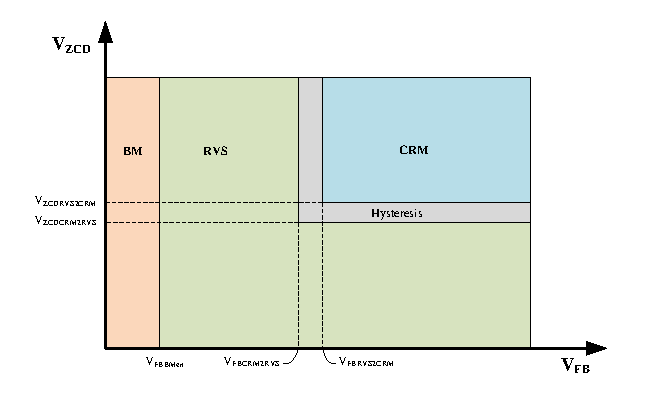
\includegraphics[width=0.6\linewidth]{figures/模式切换1.pdf}
    \caption{多模式切换图}
    \label{fig:模式切换1}
\end{figure}

本文设计了如图~\ref{fig:模式切换1}所示的多模式控制方案,模式切换通过监测引脚$V_{FB}$和引脚$V_{ZCD}$上的电压值来判断输出负载电流和输出电压的大小,一但其超过所设置的阈值,模式选择模块开始工作,切换到对应的模式。根据变换器芯片设计,当输出负载电流很小处于极轻载或空载情况时,$V_{FB}$同样小于对应的参考电压$V_{FBBMen}$,此时芯片被设定为突发工作模式;当输出负载电流逐渐增大进入轻载情况,$V_{FB}$同样随着输出负载电流的增大而增大,且其未大于$V_{FBRVS2CRM}$时,芯片工作在RVS模式中,RVS工作模式是非对称半桥反激式开关电源所特有的一种新型工作模式,能最大化地同时降低高低边功率管的开关损耗;当输出负载电流继续增大,进入重载情况后,$V_{FB}$此时大于$V_{FBRVS2CRM}$,芯片被从RVS工作模式切换为CRM工作模式,在不影响变压器中储能转换的情况下,实现最大的开关频率,最大限度地降低功率管导通损耗并为副边传递能量,维持输出电压在重载下的稳定性。为了防止模式切换时的不稳定性问题,避免芯片在两个模式中来回切换,针对性的设置了CRM模式和RVS模式之间的迟滞区间,当负载电流从重载向轻载切换时,$V_{FB}$则需要小于$V_{FBCRM2RVS}$时,才能由CRM模式切换为RVS模式。由文献可知,AHB反激式变换器系统在轻载时使用CRM模式无法达到最大的能量传递效率,因此输出电压同时制约着不同模式的切换,通过辅助绕组的分压引脚$V_{ZCD}$监测输出电压大小,根据计算和测试,选择输出电压大于15V后才允许芯片从RVS模式切换为CRM模式。为了避免模式之间的频繁切换引起的电路振荡,$V_{ZCD}$同样设置有两个偏置电压$V_{FBRVS2CRM}$和$V_{FBCRM2RVS}$作为迟滞区间。

\begin{figure}[htbp] 
    \centering
    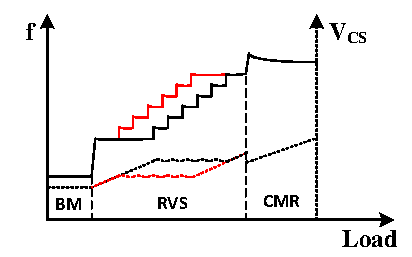
\includegraphics[width=0.6\linewidth]{figures/模式切换2.pdf}
    \caption{多模式频率变化图}
    \label{fig:模式切换2}
\end{figure}

不同的模式影响着功率管的开关频率和峰值电流变化,如图~\ref{fig:模式切换2}所示,在突发模式时,功率管开关频率处于最小值,通过使系统间歇地工作,关闭其他多余模块的工作, 降低系统的待机功耗;在RVS工作模式时,功率管开关频率随着输出负载电流的增大呈阶梯式波动,这是因为RVS模式为了减小开关损耗,只在谐振波谷的谷底处开启新的周期,开关频率非连续;在CRM工作模式时,开关频率随着输出负载电流的增大而缓慢减小,这是由于CRM模式中低边功率管由于谐振腔的原因退磁时间趋于一致,而高边功率管的导通时间随着峰值电流的增大而增大,导致周期时间相应变长,开关频率逐渐降低。

\subsection{CRM工作模式}

\subsection{RVS工作模式}

\begin{figure}[htbp] 
    \centering
    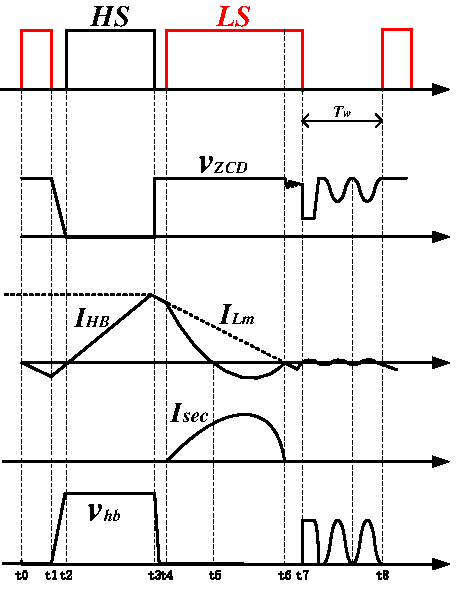
\includegraphics[width=0.6\linewidth]{figures/RVS波形图.pdf}
    \caption{RVS工作模式波形图}
    \label{fig:RVS波形图}
\end{figure}

RVS工作模式是针对非对称半桥反激式开关电源设计的一种新型的DCM操作模式,旨在轻载工况下消除高低边功率管的输出损耗。由于非对称半桥反激式变换器拓扑结构初级测和LLC型开关电源相同,存在谐振电容Cr和变压器漏感Lr组成的谐振腔,因此当控制器处于DCM控制模式时,高低边功率管都关闭的等待时间内产生谐振现象,如图~\ref{fig:RVS波形图}中Tw时间。因此无法在等待时间内利用逆向电感电流将高低边功率管中间节点电压$V_{HB}$充电到等于输入电压$V_{in}$,高边功率管存在较大的源漏电压差$V_{DS}(V_{DS}=V_{in}-V_{HB})$,故在非对称半桥反激式系统中使用传统的DCM控制方式导通高边功率管会产生巨大的开关损耗,降低电路的能量传递效率,因此非对称半桥反激式系统中一般使用边界导通(BCM)模式,BCM工作模式在重载时具有最佳的效率,在轻载时同样存在一定的问题,如能量传递延后和能量传递出现双脉冲等情况。根据文献的研究,提出了新型的谐振谷值开关工作(RVS)模式。

此控制方式巧妙地在开启高边功率管前,提前打开底边功率管一定时间,产生逆向的电感电流为$V_{HB}$节点进行充电,合理规划死区时间即可将$V_{HB}$节点电压充电到等于$V_{in}$,此时再打开高边功率管对原边电感进行励磁储能,极大的降低开关损耗和能量传递效率,具体波形图如图~\ref{fig:RVS波形图}所示。同时考虑到等待时间内$V_{HB}$的谐振情况,通过精确谷底导通模块控制低边功率管在$V_{HB}$电压谐振谷底处导通,抑制低边功率管引入的不必要的开关损耗。



\section{关键技术}
\subsection{精确谷底导通技术}
在RVS控制模式时,一个周期内存在高低边功率管都关断的等待时间阶段,此时原边电感不给副边传递能量,电感电压出现谐振现象。为了满足RVS控制模式的低开关损耗,设计精确谷底导通电路实现$V_{HB}$电压谐振谷底处导通低边功率管,减小低边功率管的开关损耗。

电路存在两个困难点,一方面是需要测量$V_{HB}$谐振电压谷底,产生对应谷底信号参与后续逻辑控制;另一方面是由于驱动电路存在的信号延时问题,会导致实际控制功率管的开关信号比PMW信号更晚产生,以致于实际低边功率管不在$V_{HB}$谐振谷底处导通,产生不必要的开关损耗。

图 是RVS模式中一个周期内$V_{HB}$信号的波形图,在等待时间内,由于原边漏感Lr和原边谐振电容Cr产生电感电容谐振;但因为$V_{HB}$电压过高无法接入芯片内进行采样处理,因此将原边电感电压通过电阻分压后产生VZCD信号传入变换器内采样。图 是VZCD电压信号的波形图,VZCD信号和$V_{HB}$信号谐振相反,$V_{HB}$的谐振谷底对应VZCD的谐振峰值。使用峰值检测电路来检测VZCD信号在等待时间内的谐振峰值,图 是峰值检测电路的电路图。再通过比较器产生峰值脉冲信号用于后续逻辑控制。

因为存在驱动器等电路的延时,为了实现精确的谷底导通功能,通过需要在$V_{HB}$谐振谷底到来之前产生低边功率管的导通逻辑信号,使得逻辑信号通过驱动器后,产生的实际控制低边功率管导通信号刚好处于$V_{HB}$信号谐振谷底的位置处,因此要求逻辑信号提前产生的时间等于驱动器等电路的延时时间。图~\ref{fig:精确谷底导通电路图1}是精确谷底导通信号的电路图。

\begin{figure}[htbp] 
    \centering
    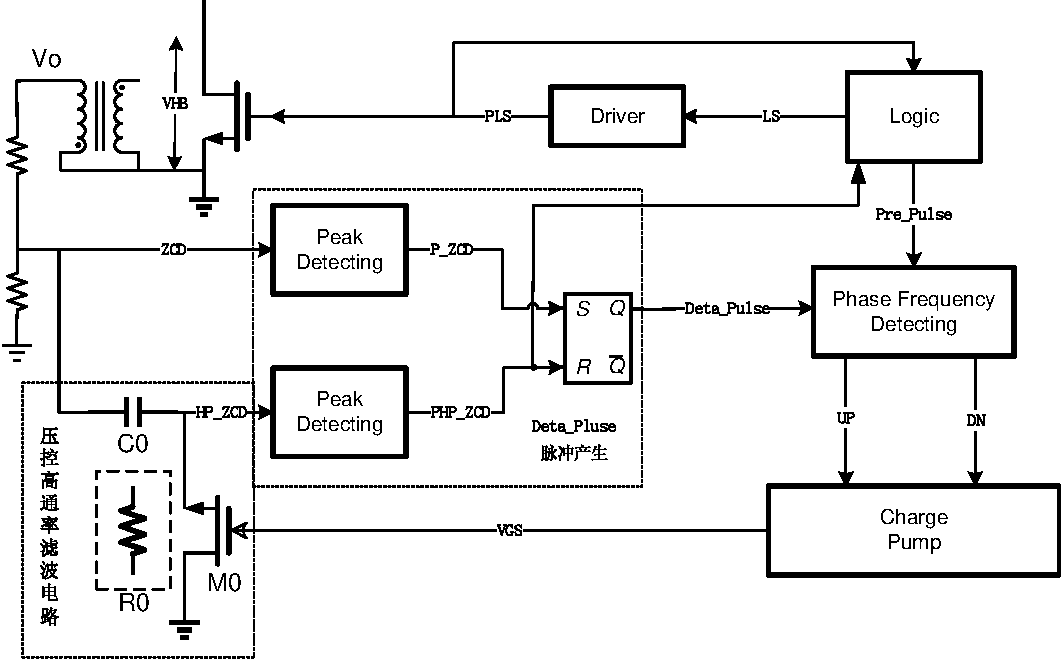
\includegraphics[width=0.6\linewidth]{figures/精确谷底导通电路图1.pdf}
    \caption{精确谷底导通电路图}
    \label{fig:精确谷底导通电路图1}
\end{figure}

LS和PLS分别是PWM控制电路产生的低边功率管控制信号和实际控制信号,通过逻辑控制电路得到LS和PLS信号的延时时间Pre\_Pulse。为了预判谷底信号,通过一个使用MOS管充当电阻的压控高通滤波器电路,产生VZCD对应的超前时间信号VHP\_ZCD,只需适当的调节VGS的大小即可控制VHP\_ZCD信号的超前时间大小。分别使用两个峰值检测电路来检测并得到两个信号的峰值脉冲信号,经过SR锁存器产生超前时间Deta\_Pulse。为了轻微的调节栅极电压信号VGS,使用了PLL电路中的鉴相鉴频器和电荷泵电路来控制Deta\_Pulse信号逐步逼近Pre\_Pulse信号,完成低边功率管的精确谷底导通功能。

\subsection{退磁时间逐步逼近技术}







